\begin{activity} \label{A:11.9.4} Let $D'$ be the region in the $xy$-plane bounded by the lines $y=0$, $x=0$, and $x+y=1$. We will evaluate the double integral
\begin{equation}
\iint_{D'} \sqrt{x+y}(x-y)^2 \, dA \label{eq:11.9.COV_ex}
\end{equation}
with a change of variables.
	\ba
	\item Sketch the region $D'$ in the $xy$ plane.
	
	\item We would like to make a substitution that makes the integrand easier to antidifferentiate. Let $s = x+y$ and $t = x-y$. Explain why this should make antidifferentiation easier by making the corresponding substitutions and writing the new integrand in terms of $s$ and $t$.

	\item Solve the equations $s = x+y$ and $t = x-y$ for $x$ and $y$. (Doing so determines the standard form of the transformation, since we will have $x$ as a function of $s$ and $t$, and $y$ as a function of $s$ and $t$.)

	\item To actually execute this change of variables, we need to know the $st$-region $D$ that corresponds to the $xy$-region $D'$.
		\begin{enumerate}[i.]
		\item What $st$ equation corresponds to the $xy$ equation $x+y=1$?
		
		\item What $st$ equation corresponds to the $xy$ equation $x=0$?
		
		\item What $st$ equation corresponds to the $xy$ equation $y=0$?
		
		\item Sketch the $st$ region $D$ that corresponds to the $xy$ domain $D'$.
			
		\end{enumerate}
		
	\item Make the change of variables indicated by $s = x+y$ and $t = x-y$ in the double integral (\ref{eq:11.9.COV_ex}) and set up an iterated integral in $st$ variables whose value is the original given double integral. Finally, evaluate the iterated integral.
	
	
	
	\ea

\end{activity}
\begin{smallhint}

\end{smallhint}
\begin{bighint}

\end{bighint}
\begin{activitySolution}
	\ba
	\item A sketch of the $xy$ domain $D'$ is shown below.
			
	\item This change of variable would make the integrand look like $\sqrt{s}t^2$, which separates the variables and makes the integration easier. 
	

	\item A little algebra shows that $x = \frac{1}{2}(s+t)$ and $y = \frac{1}{2}(s-t)$.


	\item To make this change of variables, we will need to know the $st$-region $S$ that corresponds to the $xy$-region $D$.
		\begin{enumerate}[i.]
		\item Using our change of variables we have 
\[1 = x+y = \frac{1}{2}((s+t)+(s-t)) = s.\]
	
		\item Using our change of variables we have 
\[0 = x = \frac{1}{2}(s+t)\]
or
\[s+t = 0.\]		
		\item Using our change of variables we have 
\[0 = y = \frac{1}{2}(s-t)\]
or
\[s-t = 0.\]
	
		\item The region $D$ is shown below. 
		
		\end{enumerate}
		
	\item We need the Jacobian
\[\left|\frac{\partial(x,y)}{\partial(s,t)}\right| = \left|\frac{\partial x}{\partial s} \frac{\partial y}{\partial t} - \frac{\partial x}{\partial t} \frac{\partial y}{\partial s}\right| = \left| \left(\frac{1}{2}\right)\left(-\frac{1}{2}\right) - \left(\frac{1}{2}\right)\left(\frac{1}{2}\right)\right| = \frac{1}{2}.\]
Then
\begin{align*}
\iint_D \sqrt{x+y}(x-y)^2 \, dA &= \iint_S \sqrt{s}t^2 \left|\frac{\partial(x,y)}{\partial(s,t)}\right| \, ds \, dt \\
	&= \int_0^1 \int_{-s}^{s} \sqrt{s}t^2 \frac{1}{2} \, dt \, ds \\
	&= \frac{1}{2} \int_0^1 \left. \sqrt{s} \frac{t^3}{3} \right|_{-s}^{s} \, ds \\
	&= \frac{1}{3} \int_0^1 \sqrt{s}s^3 \, ds \\
	&= \frac{1}{3} \int_0^1 s^{7/2} \, ds \\
	&= \frac{2}{27} \left. s^{9/2} \right|_0^1 \\
	&= \frac{2}{27}.
\end{align*}
	\ea
\begin{center}
\resizebox{!}{1.5in}{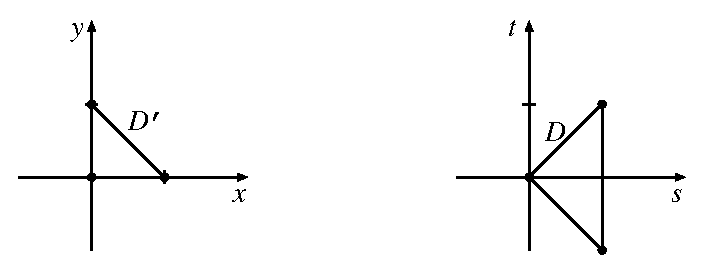
\includegraphics{11_9_Act_4}}
\end{center}
\end{activitySolution}
\aftera
